\section{Proposal}\label{sec:prop}
% Proposal:
%  - retomar problema {iot, sec, ND};
%  - objetivo;
%  - soluções {minas, paralelismo, distribuído, ~~py-kafka, flink,~~ mpi}
%  - propor uma solução

Amid of \iot expansion in multiple fields, from industry to daily life,
the constant threat of intrusion, subversion (overthrow), denial of service
or any other unexpected detrimental behavior by any component of a system or
external actors is a prospect looming over many systems administrators.
Following that reasoning, new \nids and other autonomous and analytics system
surveillance tools are being proposed, many employing technics such as Anomaly
and Novelty Detection.

These tools require the network packet traffic to be constantly analysed,
aggregated into flow descriptors and further processed in a classification
and any Intrusion Detection.
This requirement in turn, requesting more computing power at the edge.
While requesting more computing power in a cloud environment is trivial and
inexpensive, the same cannot be said 

\begin{highlight}
Fog computing infrastructure aims to offload
computing resources from cloud providers by placing edge
devices closer to end-users and/or data sources.

Objective: Distributed novelty detection in streams using limited hardware.

Previous attempts to attain the objective of distributed fast
\end{highlight}

The overall organization of components, connections and interactions with external
actors is shown in \reffig{mfog-phy-arch-cloud},
from bottom left to top right: sensor network; fog containing gateway router
and novelty detection cluster; cloud storage for model, alarms and statistics
and; human supervisor addressing alarms and statistics.

\begin{figure}[hbt]
  \centering
  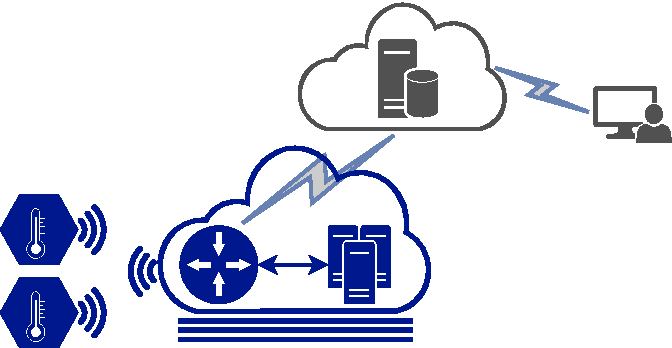
\includegraphics[width=0.9\linewidth,page=1]{figures/mfog-arch-fisica.svg.pdf}
  \caption{\mfog physical architecture overview with cloud model storage.}
  \label{fig:mfog-phy-arch-cloud}
\end{figure}